% Andrew G. West - prop_spec.tex
% Main LaTeX file for CIS400/401 Project Proposal Specification
%

\documentclass{sig-alternate}
 
\usepackage{mdwlist}
\usepackage{url}

\begin{document} 

% AW - We setup the parameters to our title header before 'making' it.
\title{CIS400/401 Project Proposal Specification - BartenderBot}
\subtitle{Dept. of CIS - Senior Design 2010-2011}
\numberofauthors{3}
\author{
\alignauthor Seth Shannin \\ \email{sshannin@seas} \\ Univ. of Pennsylvania \\ Philadelphia, PA
\alignauthor Kevin Xu \\ \email{kevinxu@seas} \\ Univ. of Pennsylvania \\ Philadelphia, PA
\alignauthor Camillo Jose Taylor \\ \email{cjtaylor@cis} \\ Univ. of Pennsylvania \\ Philadelphia, PA}
\date{}
\maketitle

\begin{abstract}
\textit{Programming a robot to perform human tasks has been the focus of many research papers. The task has been traditionally very challenging, as it involves heavy computation and complicated coordination between many different joints. Here we present a method to teach the Willow Garage PR2 robot how to mix and serve a drink through imitation. By using immersive teleoperation, it is possible to issue complex commands to the PR2 and have it shadow human motion. The teleoperation will be provided by the Microsoft XBox Kinect, and communication with the PR2 will be handled with ROS. The goal of this project is to have the PR2 not only shadow human motion captured by the Kinect, but also learn from this motion and adapt to new situations via reinforcement learning techniques. We will outline our plan for achieving both shadowing and learning with the Kinect, PR2, and ROS.}
\end{abstract}

	% AW - Then we proceed into the body of the report itself. The effect of the 'section' command is obvious, but also notice 'label'. Its good practice to label every (sub)-section, graph, equation etc. -- this gives us a way to dynamically reference it later in the text via the 'ref' command.
\section{Introduction}
\label{sec:intro}
Constructing a fully autonomous and adaptive robot has been a long-time goal of robotics research. There have been many different attempts at overcoming the challenges involved in developing such a robot. The ability to learn is a powerful intermediate step towards full autonomy. A common problem involves choosing how exactly to demonstrate a desired behavior in such a way that a robot can learn that behavior. In this paper we propose to teach a WillowGarage PR2 Robot how to perform a reasonably complex task (mixing a drink) through shadowing of human motion capured by the Microsoft XBOX Kinect. The XBOX Kinect sensor from Microsoft provides real-time depth information from a scene at 30 FPS. Combined with various open source libraries\cite{kinect}, the Kinect has been used in many projects involving real-time tracking of human motion, many of which can be found online\cite{freenect}. The PR2 is a humanoid robot developed by  Willow Garage\cite{pr2} for the purpose of robotics research. It  has been taught by different teams to do many things, including baking cookies\cite{cookies}, scanning and bagging groceries\cite{groceries}, and fetching a sandwich from Subway\cite{subway}.

We propose to use the Kinect to map human movement to teach the PR2 how to mix and pour a drink. The Kinect sensor provides a convenient way to demonstrate the desired behavior by tracking human motion. The captured data can be relayed to the PR2 via ROS, an open-source Robot Operating System\cite{ros}. ROS provides a convenient framework for inter-process communication and coordination between different sensors and components of the PR2. ROS enables relatively short programs to issue surprisingly sophisticated commands to the PR2, such as continually tracking a moving point over time\cite{ros_pr2}. By using ROS, Kinect, and the PR2, we will demonstrate the effectiveness of teleimmersive demonstration learning in teaching a robot new behavior.

This method has several advantages over existing approaches. First of all, the Kinect sensor provides accurate real-time human motion tracking that can be translated to joint movement in the PR2 thanks to ROS. Secondly, teleimmersion better enables a human teacher to show a robot learner exactly how to move in a given situation compared to kinesthetic learning, which involves manipulating the robot learner directly by physical contact. Teleimmersion will also allow demonstrations for robots that cannot be subject to kinesthetic learning easily, such as very large or very small robots. Our method, if successful, would allow for rapid introduction of all kinds of different behavior to the PR2 all from human motion. This technique could be generalized to other humanoid robots besides the PR2 to teach them different behavior.
	
\section{Related Work}
\label{sec:related_work}
There have been many other projects involving autonomous robots and handling drinks. Hillenbrand \textit{et al.}~\cite{pouring_arm} designed a semi-autonomous hand-arm robot for serving drinks. The robot was capable of responding to user input by choosing a drink from multiple choices, opening it, and pouring it into a glass, and then offering the drink to the user. The hand was capable of not only picking up bottles and cups, but also unscrewing bottle caps. The robot combined stereo processing and object recognition to identify the drinks, and then used grasp planning to pick up the drink itself. Bohren \textit{et al.}~\cite{beer} used the PR2 and ROS to build a robotic system for retrieving a beer from a refrigerator. In their work, they developed a task-level execution system known as SMACH for rapidly prototyping robotic applications. The PR2 had to navigate an obstacle map to reach the refrigerator, use object recognization and grasp planning to identify the door handle and the drinks, and ultimately use facial recognition to deliver the beer to a human recipient. Each step of the process contained detail planning and image processing in order to carry out the expected behavior. Srinivasa \textit{et al.}~\cite{herb} designed an autonomous robot capable of navigating a household-like environment and manipulating a wide variety of household objects. Consisting of an arm mounted on a segway, HERB used a powerful array of six multi-core processors to successfully traverse its environment and interact with objects around it.

All of these robots relied on vision processing and path planning to carry out their tasks. However, there have been other approaches involving demonstration and learning to allow a robot to perform a specific job. Kormushev \textit{et al.}~\cite{walk_imitation} taught a robot new motor skills through kinesthetic teaching. The robot had two distinct modes of operation: a learning phase and a reproduction phase. During the learning phase, the robot was shown how to clean a whiteboard by direct human manipulation of the robot's joints, recording both position and force information. During the reproduction phase, the robot would translate the learned information to its own reference frame and attempt to duplicate the teacher's movement pattern on the whiteboard.  Kormushev \textit{et al.}~\cite{pancakes} also used kinesthetic learning to teach a robotic arm how to flip a pancake. A human teacher first moved the arm to demonstrate the movement required to flip a pancake 180 degrees in the air and catch it again. In subsequent trials, reinforcement learning techniques were applied such that the robot could evaulate the performance of its flips and attempt to adjust the motion of the arm for better future flips. In a much earlier attempt, Chalodhorn \textit{et al.}~\cite{walk_imitation} used motion capturing to teach a bipedal humanoid robot how to walk by imitation. Joint angles from motion capture data from a human demonstrator wearing a motion capture suit were mapped to joint angles in the robot. This data was combined with predictions of future state based on sensory information to reproduce a human-like gait in the robot. 

\section{Project Proposal}
\label{sec:project_proposal}We propose to teach a PR2 robot to mix drinks via
teleimmersive demonstration learning methods. It is our goal that given a 
setting consisting of bottles and glasses, the PR2 will be able to select
desired bottles and pour them into glasses, just by having seen a human
trainer perform these actions in the past.

\subsection{Anticipated Approach}
\label{subsec:approach}
At the base level, the hardware layer of the PR2 will be managed by ROS.
Using the mounted Kinect, the PR2 will observe a human trainer go
through the process of selecting bottles and pouring them into glasses. Custom 
software will then attempt to map the motions of the human trainer onto the 
motor system of the PR2.
\\
\\After this training, the PR2 will begin putting its learned motions to test.
It will be asked to select various bottles and  pour different combinations of
drinks under a reinforcement-learning system.
\\
\\ROS is a fairly mature and ubiquitous piece of software and will take care of
many of the more sophisticated computational tasks (such as path planning, 
image segmentation, etc.) that we would otherwise have to devote significant 
amounts of time to developing.  
Likewise, we intend to make heavy use of the Kinect API, which comes with very
strong support for human joint detection.
While we expect both ROS and Kinect to have relatively steep learning curves,
we do not anticipate these being the limiting factor in how much progress we
are able to achieve. 
Rather, we expect the area of novel difficulty to be the combining of these
two distinct systems into one coherent system which can be used for
teleimmersive learning.

\subsection{Evaluation Criteria}
\label{subsec:eval_criteria}
We will evaulate the performance of our proposed system to teach the PR2 by experimentally determining how quickly and easily the PR2
can acquire new behavior. We will start with very simple motions, such as simply lifting and pouring a single cup or bottle. Once the PR2 is capable of completing those actions after shadowing a human demonstrator, we can attempt to teach it increasingly complex sequences of mixing and pouring. The goal here is to show that many different movement sequences can be taught to the PR2 using the same motion capturing setup from the Kinect.

If time permits, we would also like to evaluate the PR2's ability to adapt to changing conditions. For instance, we can measure how far a bottle can be moved from its expected position before the PR2 becomes unable to pick it up. The weight of the bottle can also be toggled to see how well the PR2 can adapt to nearly-full versus nearly-empty drink containers.

\section{Research Timeline}
\label{sec:research_timeline}
The following is a list of milestones we hope to reach as the fall and spring semesters progress. 

	% The 'itemize' environment shown here, and its friend 'enumerate' (shown below), are used to create indented\bulleted\outline style lists.
\begin{itemize*}
	\item {\sc already completed}: Preliminary reading and project selection. Project proposal completed.\vspace{3pt}
	\item {\sc prior-to Nov.1}: Complete ROS tutorials and practice using ROS.\vspace{3pt}
	\item {\sc prior-to Dec.1}: Capture human movement with Kinect. Experiment with PR2 simulator.\vspace{3pt}
	\item {\sc prior-to winter break}: Issue commands to PR2 simulator by human gestures captured by Kinect. Progress report completed.\vspace{3pt}
	\item {\sc prior-to Feb.1}: Attempt real trials on the actual PR2.\vspace{3pt}
	\item {\sc prior-to Mar.1}: Achieve a simple, successful drink mixing with the PR2.\vspace{3pt}
	\item {\sc prior-to Apr.1}: Develop a more complex sequence of drink mixing with the PR2.\vspace{3pt}
	\item {\sc completion tasks}: Verify that the PR2 can successfully mix a drink. Conduct accuracy testing. Complete write-up.\vspace{3pt}
	\item {\sc if there's time} : Investigate ways to improve the PR2's ability to adapt and learn from different drink configurations.
\end{itemize*}

	% AW: We next move onto the bibliography.
\bibliographystyle{plain} % Please do not change the bib-style
\bibliography{prop_spec}  % Just the *.BIB filename

	% AW: Here is a dirty hack. We insert so much vertical space that the appendices, which want to begin in the left colum underneath "references", are pushed over to the right-hand column. If we looked hard enough, there is probably a command to do exactly this (and wouldn't need tweaked after edits).
\vspace{150pt}

	% AW: We then use appendices to share some additional information with you, though you won't need appendices in your own proposal.
\appendix
\section{Other Specifics}
\label{app:other_specifics}
Your proposal need not have appendices like this section and the next, but we still have critical info to share:

	% The usage of 'enumerate' (similar to 'itemize') we talked about above
	%
	% You may also notice we have many 'vspace' commands lying around. These create 'vertical space' and are a way to force LaTeX to cooperate, sometimes. Don't get too involved with using them initially, though, because adding or deleting a single line of task can dramatically change how LaTeX chooses to format, page, and space the document
\begin{enumerate*}
	\item {\sc proposal length}: We require that your proposal be 4--5 pages in length, bibliography included. Be careful, \LaTeX{} and our style-file in particular are \textit{extremely} space efficient. An 9-page MS-Word document could easily become a 5-page \LaTeX{} one.\vspace{5pt}
	\item {\sc plagarism}: \textbf{DO NOT} plagarize. If you are caught, you will fail the class (\textit{i.e.}, not graduate), or worse. 
\end{enumerate*}

\section{\LaTeX{} Examples}
\label{app:latex_examples}

	% This paragraph makes use of dynamic references. Remember how we've been 'label'-ing everything; sections, etc? Using 'ref' we can reference them. Add a new figure/section at the beginning? This technique automatically re-numbers when you build, so you don't have to make static changes.
At this point, the proposal specification is complete. From here on out, we are just going to show off some commonly used \LaTeX{} technique. Be sure to look at the `code behind' and see Tab.~\ref{tab:some_table}, Eqn.~\ref{eqn:some_equation} and Fig.~\ref{fig:some_graph} for the output!

	% AW - We next encounter tables and figures (images). Big things like these are known as 'floats' in LaTeX because their position is not fixed. Notice that '[htb!]' follows the start of each environment. We are telling LaTeX that we'd like to put the table/fig 'h' - HERE, precisely where it follows in the narrative. If LaTeX determines it doesn't look good here, 't' tells LaTeX we'd like it at the top of this column, and if that doesn't work, use 'b', the bottom of the column. Other options are available. LaTeX shifts floats around to ensure images don't end up on page/column boundaries, which would result in a waste of space for text.

	% AW - We insert a graph/figure into the document. This is a pretty straightforward process once you get the image into a file format that LaTeX plays nice with. Then we just scale it as a % of the column width.
\begin{figure}[htb!]
	\begin{center}
		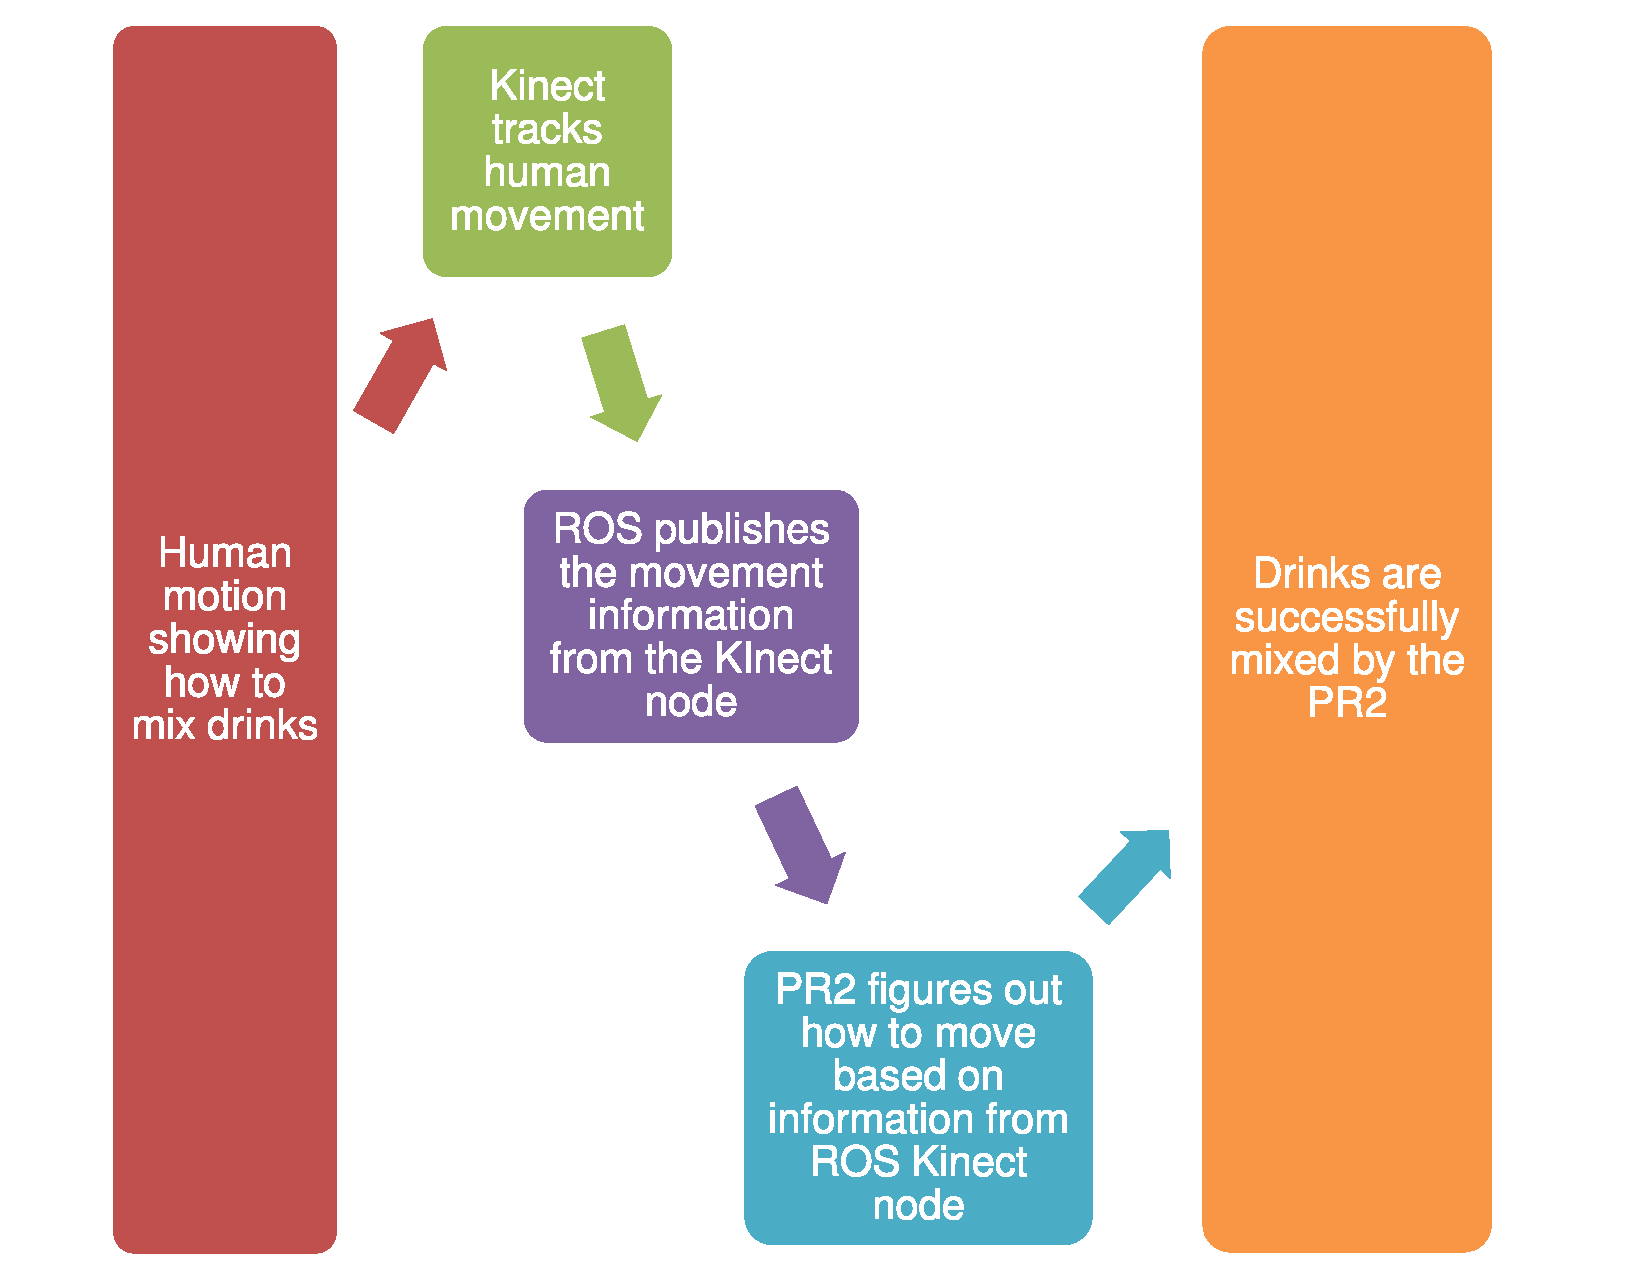
\includegraphics[width=0.9\linewidth]{flowchart}
	\end{center}
	\vspace{-12pt}
	\caption{Block Diagram detailing Anticipated Approach}
	\label{fig:some_graph}
\end{figure}

\end{document} 

